\input{preamble.tex}

\begin{document}
	\setcounter{page}{1}
	
	\begin{center} 
		\textbf{Правительство Российской Федерации}
		\\ \textbf{Федеральное государственное автономное образовательное учреждение}
		\\ \textbf{высшего профессионального образования}
		\\ \textbf{«Национальный исследовательский университет»}
		\\ \textbf{«Высшая школа экономики»}
		\\ \textbf{Нижегородский кампус}
		\vspace{3cm}
		\\ Факультет математики, информатики и компьютерных наук
		\\ Кафедра фундаментальной математики
		\vspace{3cm}
		\\ \large\textbf{ВЫПУСКНАЯ КВАЛИФИКАЦИОННАЯ РАБОТА}
		\vspace{0.3cm}
		\\ \large\textbf{РЕАЛИЗАЦИЯ И СРАВНИТЕЛЬНЫЙ АНАЛИЗ ОПТИМИЗИРОВАННЫХ АЛГОРИТМОВ КРАСКАЛЛА И ПРИМА}
	\end{center}
	
	\vspace{2cm}\hspace{8cm} Выполнил: 
	\par \hspace{8cm} Студент 4 курса группы 22 ФМ 
	\par \hspace{8cm} Турсунов Данил Вячеславович
	\par \vspace{0.8cm} \hspace{8cm} Научный руководитель:
	\par \hspace{8cm} Малышев Дмитрий Сергеевич
	\begin{center} 
		\vspace{3cm} Нижний Новгород
		\par Май 2026 г.
	\end{center}
	\newpage
	
	\tableofcontents
	\newpage

	\section{Введение}
	
	\subsection{Основные определения}
	
	\hspace{0.5 cm}
	
	В данной работе будут рассматриваться алгоритмы, решающие задачу построения минимального остовного дерева по заданному связному неориентированному взвешенному графу.
	
	Перед описанием непосредственно рассматриваемой задачи и алгоритмов, с помощью которых эта задача решается, дадим определения основным понятиям, фигурирующим в работе:
	
	\begin{definition} (Конечный граф) $\\$
		Конечным графом называется упорядоченная пара (V,E), для которой выполнены следующие условия:
		\par 1) V - непустое конечное множество вершин;
		\par 2) E - множество пар вершин, называемых рёбрами.
	\end{definition}
	\begin{definition} (Неориентированный граф) $\\$
	Неориентированный граф - граф, в котором рёбра не имеют направления, то есть $E$ состоит из неупорядоченных пар $\{u, v\}$.
	\end{definition}
	\begin{definition} (Взвешенный граф) $\\$
	Взвешенный граф - граф, в котором каждому ребру присвоен числовой вес.
	\end{definition}
	\begin{definition} (Инцидентность) $\\$
		Если граф содержит ребро e = (a,b), то каждую из вершин a, b называют инцидентной ребру e и говорят, что вершины a и b соединены ребром e.
	\end{definition}
	\begin{definition} (Путь в графе) $\\$
		Путём в графе называют конечную последовательность его вершин и рёбер вида: $b_0, (b_0, b_1), b_1, \dots, b_{i-1}, (b_{i-1}, b_{i}), b_{i}, \dots, b_{k-1}, (b_{k-1}, b_{k}), b_{k}, k >= 1$. Число k называется длиной пути, оно совпадает с числом входящих в него рёбер.
	\end{definition}
	\begin{definition} (Связность графа) $\\$
	Граф называют связным, если любые две его вершины можно соединить путём.
	\end{definition}
	\begin{definition} (Цикл в графе) $\\$
		Циклом длины $k \in \mathds{N}$ в графе называют конечное подмножество его вершин и рёбер вида \{$b_0, (b_0, b_1), b_1, \dots, b_{i-1}, (b_{i-1}, b_{i}), b_{i}, \dots, b_{k-1}, (b_{k-1}, b_{0})$\}. Простым циклом называют цикл, у которого все вершины и рёбра попарно различны.
	\end{definition}
	\begin{definition} (Дерево) $\\$
	Дерево --- cвязный неориентированный граф без циклов.
	\end{definition}
	\begin{definition} (Остовное дерево) $\\$
	Для связного неориентированного графа \( G = (V, E) \) остовное дерево \( T = (V, E') \) --- это подграф, удовлетворяющий условиям:
	\par 1) \( T \) является \textit{деревом},
	\par 2) \( V(T) = V(G) \) (содержит все вершины исходного графа),
	\par 3) \( E' \subseteq E \) (рёбра принадлежат исходному графу).
	\end{definition}
	\begin{definition} (Минимальное остовное дерево) $\\$
	Для взвешенного связного неориентированного графа $G$ минимальное остовное дерево --- это остовное дерево $T \subseteq G$, такое что сумма весов рёбер $T$ минимальна среди всех возможных остовных деревьев,
	\end{definition}
	
	\begin{definition} (Асимптотическая сложность) $\\$
		Асимптотическая сложность алгоритма --- это функция $f(n)$, которая описывает рост количества элементарных операций при увеличении размера входных данных $n \to \infty$, игнорируя константные множители и слагаемые младшего порядка.
	\end{definition}
	
	\begin{definition} (O-большое) $\\$
		Говорят, что $f(n) = O(g(n))$, если существует константа $c$ и пороговое значение $n_0$, такие что для всех $n \ge n_0$ значение $f(n)$ не превосходит $c \cdot g(n)$. \\
		$O(g(n)) = \{ f(n) \mid \exists\, c > 0,\ n_0 > 0 : 0 \le f(n) \le c \cdot g(n) \ \forall n \ge n_0 \}$.
	\end{definition}
	
	В дальнейшем под словом ``граф'' будем понимать связный неориентированный взвешенный граф.
	
	В работе часто упоминаются термины, имеющие различный смысл в математике и в программировании. Примером такого термина может служить вектор.
	
	Вектор - это динамический массив из стандартной библиотеки языка программирования C++. Основной его особенностью является возможность добавления элемента в конец и удаление элемента из конца с амортизированной асимптотической сложностью O(1). Принцип работы вектора подробно изложен в [ГДЕ].
	
	\subsection{Алгоритмы решения задачи}
	\hspace{0.5 cm}Алгоритм поиска минимального остовного дерева насчитывает практически вековую историю: в 1920-х годах правительство Чехословакии столкнулось с проблемой электрификации сельской местности, требовалось соединить все деревни электросетью, потратив минимальное количество средств. Здесь и появляется аналогия с вершинами и рёбрами: вершины - деревни, рёбра - стоимость прокладки кабеля.
	
	И в 1926 году чешский математик Отто Борувка, решая этот вопрос, впервые описал алгоритм поиска минимального остовного дерева, который впоследствии стал называться алгоритмом Борувки. Однако его работа не получила широкого распространения, и только в 1950-х годах, с активным развитием теории алгоритмов, учёные Прим и Краскалл разработали собственные алгоритмы нахождения минимальных остовных деревьев. Эти алгоритмы и будут рассмотрены в курсовой работе.
	
	В 1956 году Джозеф Краскал опубликовал собственный алгоритм нахождения минимального остовного дерева. Основная идея алгоритма заключается в использовании системы непересекающихся множеств для проверки связности текущего дерева и, в случае несвязности, добавления минимального ребра к текущему дереву.
	
	В 1957 году Роберт Прим независимо от него разработал собственный алгоритм, решая задачу прокладки телефонных кабелей. Основная идея алгоритма - пошаговое увеличение дерева за счёт добавления рёбер, инцидентных добавленной вершине и недобавленной вершине, с минимальным весом, при этом рёбра с минимальным весом хранятся в различных структурах данных, позволяющих хранить расстояние от строящегося дерева до недобавленных вершин и возвращать номер ближайщей вешины. Примечательно, что алгоритм Прима практически полностью совпадает с алгоритмом Дейкстры, который решает задачу поиска минимального пути; единственное различие заключается в выборе ребра: в алгоритме Дейкстры ребро выбирается по суммарному пути.
	
	\newpage
	
	\subsection{Описание работы}
	
	\hspace{0.5 cm} Выпускная квалификационная работа представляет собой написание программы (кода), которая состоит из 2-х частей: алгоритмической и аналитической. Изначально запускается алгоритмическая часть кода, которая написана на языке программирования C++, в ней реализованы следующие подпрограммы:
	
	- алгоритм Краскала;
	
	- система непересекающихся множеств;
	
	- алгоритм Прима;
	
	- стратегия алгоритма Прима на векторе;
	
	- стратегия алгоритма Прима на двоичной приоритетной очереди;
	
	- стратегия алгоритма Прима на фибоначчиевой приоритетной очереди;
	
	- генератор графов;
	
	- итоговая подпрограмма, которая генерирует графы различного количества вершин и рёбер и запускает на них алгоритмы Краскалла и Прима со всеми оптимизациями, измеряя время построения минимального остовного дерева и выводя в отдельные файлы (для каждой пропорции количества рёбер и количества вершин создаётся отдельный файл) количество вершин, количество рёбер и время работы алгоритма.
	
	Далее запускается аналитическая часть, состоящая из двух подпрограмм, каждая из которых берёт информацию из файлов, сгенерированных алгоритмической частью:
	
	- программа, проводящая сравнительный анализ скорости работы алгоритмов Краскалла и Прима вместе с оптимизациями. Она строит отдельный график времени, потребовавшегося на построение минимального остовного дерева, в зависимости от количества вершин для каждой пропорции количества рёбер и количества вершин;
	
	- программа, строящая графики отношения времени выполнения алгоритмов Краскалла и Прима к оценке их асимптотической сложности.
	
	В следующих главах подробно рассматривается каждая подпрограмма алгоритмической части отдельно, кроме генерации графов, которая по смыслу больше подходит к аналитической части.
	
	\section{Алгоритм Краскалла и система непересекающихся множеств}
	
	\subsection{Алгоритм Краскалла}
	
	\hspace{0.5 cm}
	
	Алгоритм Краскала строит минимальное остовное дерево поэтапно, добавляя рёбра исходного графа к графу, не содержащему рёбер, в порядке возрастания их весов. Ребро добавляется только в том случае, если оно соединяет вершины, принадлежащие разным компонентам связности строящегося графа.
	
	Алгоритм Краскала реализован в виде функции Kruskal, которая принимает на вход граф, заданный списком рёбер, а возвращает граф в виде списка смежности и время работы алгоритма. Различие входного и выходного представлений обусловлено тем, что для работы алгоритма необходима сортировка рёбер по возрастанию, которую неудобно выполнять при использовании списка смежности.
	
	В написанной программе функция Kruskal работает следующим образом: сначала создаётся пустой граф, который по завершении алгоритма станет минимальным остовным деревом, а исходный список рёбер сортируется по возрастанию весов. Затем начинается непосредственное выполнение алгоритма Краскала: все рёбра перебираются от меньшего к большему, и если очередное ребро соединяет вершины, ещё не связанные путём в строящемся графе, то это ребро добавляется в граф. После завершения цикла полученный граф возвращается в виде списка смежности. По окончании работы алгоритма построенный граф является минимальным остовным деревом исходного графа. Корректность алгоритма доказана в [ГДЕ].
	
	Важно отметить, что проверка на то, соединяет ли ребро вершины, не связанные путём в строящемся графе, не является тривиальной и производится при помощи системы непересекающихся множеств.
	
	\subsection{Пример работы алгоритма Краскалла}
	
	\begin{figure}[htbp]
		\centering
		\	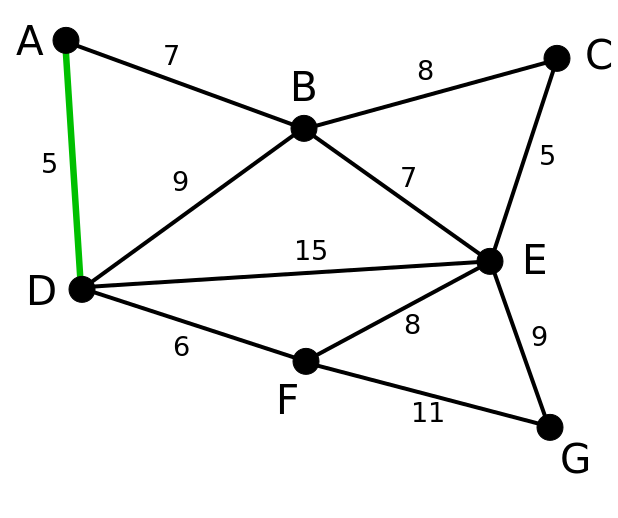
\includegraphics[width=0.3\textwidth]{images/example_kruskal/kruskal_1.png}
		\hfill
		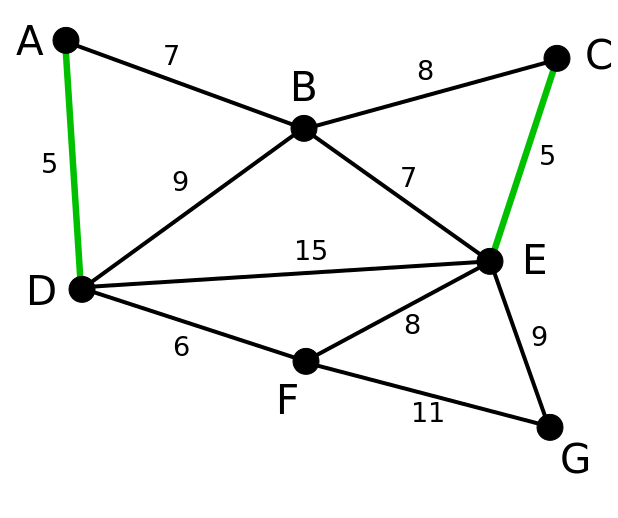
\includegraphics[width=0.3\textwidth]{images/example_kruskal/kruskal_2.png}
		\hfill
		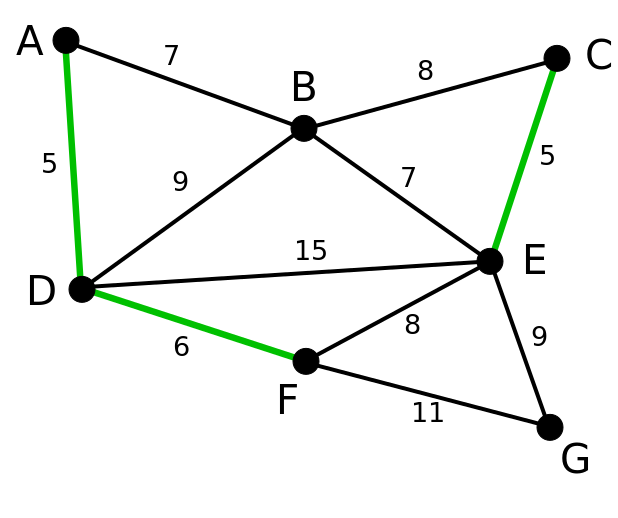
\includegraphics[width=0.3\textwidth]{images/example_kruskal/kruskal_3.png}
	\end{figure}
	\begin{figure}[htbp]
		\centering
		\	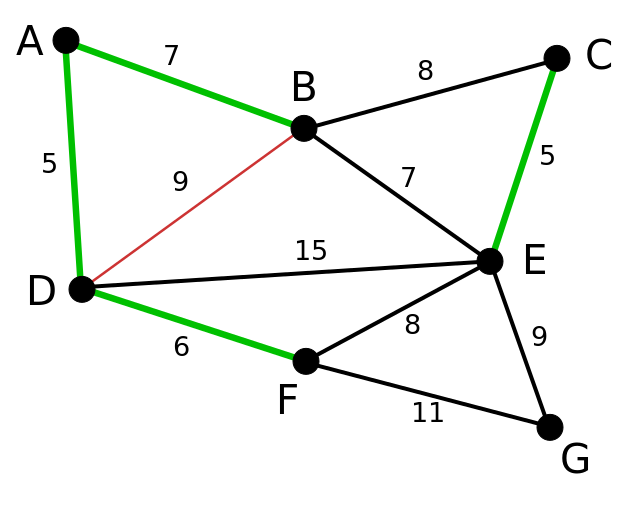
\includegraphics[width=0.3\textwidth]{images/example_kruskal/kruskal_4.png}
		\hfill
		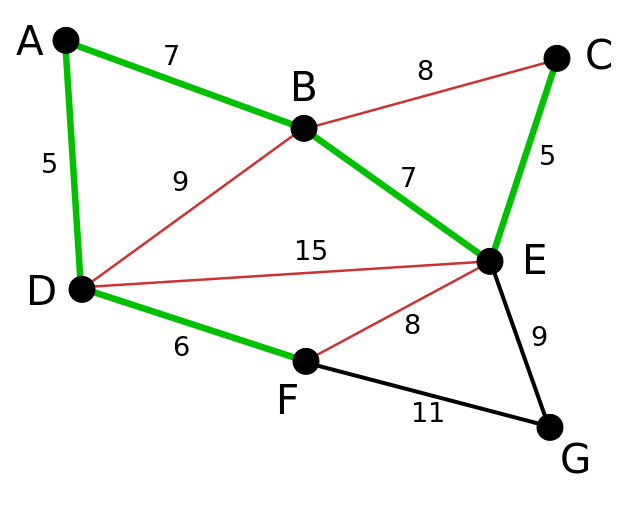
\includegraphics[width=0.3\textwidth]{images/example_kruskal/kruskal_5.png}
		\hfill
		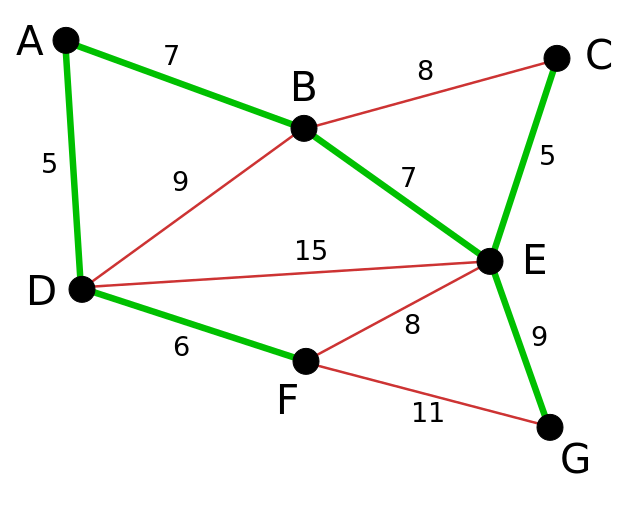
\includegraphics[width=0.3\textwidth]{images/example_kruskal/kruskal_6.png}
		\caption{Пример работы алгоритма Краскалла (6 шагов)}
	\end{figure}
	
	\subsection{Система непересекающихся множеств}
	
	\hspace{0.5 cm} Перед описанием системы непересекающихся множеств вспомним основную идею алгоритма Краскала: после сортировки всех рёбер исходного графа по весу начинается перебор рёбер от меньшего к большему. В случае, если ребро соединяет вершины, которые в новом графе принадлежат различным компонентам связности, ребро добавляется в новый граф. В противном случае ребро не добавляется, происходит переход к следующему ребру.
	
	Ключевым моментом является проверка на то, соединяет ли ребро вершины из разных компонент связности. Наивное решение этой задачи для каждой такой проверки запускало бы поиск в глубину, алгоритмическая сложность такого решения составляет $O(V + E)$, что привело бы к общей теоретической сложности алгоритма Краскала $O(VE + E^{2})$.
	
	Для более оптимального решения этой задачи требуется структура данных, которая могла бы достаточно быстро проверять, лежат ли вершины в одной компоненте связности, и делать из двух конкретных компонент связности одну после добавления ребра. Имеет смысл решать более общую задачу, рассматривая не компоненты связности, а множества. 
	
	Примером такой структуры данных может являться система непересекающихся множеств (СНМ). Она представляет из себя структуру данных, в которой хранится вектор предков вершин. Индексами этого вектора являются номера вершин. Вершина, считающая предком себя, называется представителем множества. Изначально каждая вершина является представителем множества, потому что новый граф представляет из себя набор вершин без рёбер. В программе СНМ реализована как класс DSU (disjoint-set union), вектор предков имеет название parent.
	
	Система непересекающихся множеств является иерархической структурой, где каждое множество является деревом. Поэтому, чтобы объединить 2 множества вершин $x$ и $y$, необходимо сделать следующее:
	1) найти представителей множеств вершин $x$ и $y$;
	2) у одного из представителей указать предком другого представителя, другими словами, подвесить одну вершину к другой, что поддерживает иерархическую структуру.
	
	Поиск представителей происходит рекурсивно: найти представителя вершины $x$ --- это представитель вершины-предка $x$. Если вершина считает предком саму себя, то она является представителем множества. В коде данную задачу выполняет метод find\_parent, который принимает на вход номер вершины $x$.
	
	Поиск представителей можно оптимизировать, используя эвристику спрямления путей. Она заключается в том, чтобы на обратном пути из рекурсии всем промежуточным вершинам обновить предка на представителя. Тогда при последующих прохождениях не придётся проходить через промежуточные вершины, через которые мы проходили раньше, что существенно ускоряет время работы программы.
	
	Подвешивание одной вершины к другой реализуется тривиально, однако нетривиальным остаётся способ выбора той вершины, к которой будут подвешивать другую. Для этого в структуре данных содержится вектор, который хранит в себе размеры множества. Стоит отметить, что корректные размеры множества хранятся только у вершин-представителей, потому что другие вершины подвешиваться больше не будут. Теперь будем подвешивать другую вершину к той, у которой больше размер множества. В противном случае могут возникать высокие деревья, что делает поиск представителя достаточно долгим. В программе данную задачу выполняет метод unite, который принимает на вход 2 номера вершин $x$ и $y$. Вектор размеров имеет название size. 
	
	Итоговая теоретическая сложность объединения двух множеств будет равняться $O(\alpha (V))$, где $\alpha (V)$ --- обратная к функции Аккермана. Эта функция растёт очень медленно, поэтому при оценке общей скорости работы её принимают за константу. После внедрения СНМ в работу алгоритма, общая оценка сложности работы алгоритма Краскала составит $O(E log E)$.
	
	В реализации алгоритма Краскала СНМ используется следующим образом: после сортировки всех рёбер по возрастанию создаётся экземпляр класса DSU, названный dsu. Далее, при проходе цикла по всем рёбрам, пусть у рассматривается ребро edge(from, to, cost). Если dsu.find\_parent(from) не равен dsu.find\_parent(to), то вызывается dsu.unite(from, to). После окончания цикла все множества объединяются в одно, а функция, реализующая алгоритм Краскала, возвращает получившийся граф.
	
	Пример работы системы непересекающихся множеств приведён на рисунке [ДОБАВИТЬ РИСУНОК].
	
	\section{Алгоритм Прима и приоритетные очереди}
	
	\subsection{Алгоритм Прима}
	
	\hspace{0.5 cm}
	
	Алгоритм Прима заключается в жадном построении минимального остовного дерева. Дерево строится поэтапно: на каждой итерации к построенной части дерева добавляется очередное ребро. Жадность заключается в том, что на каждой итерации алгоритма для добавления в строящееся дерево выбирается минимальное ребро из тех, что соединяет произвольную недобавленную вершину и произвольную добавленную.
	
	В коде логику алгоритма Прима реализует функция \texttt{Prim\_generic}, которая соответствует паттерну проектирования "Стратегия". Функция принимает на вход исходный граф и стратегию, а возвращает получившееся минимальное остовное дерево и время работы алгоритма для дальнейшего анализа. 
	
	Принимаемые на вход стратегии соответствуют дальнейшим оптимизациям алгоритма Прима, они описаны в пункте [В КАКОМ ПУНКТЕ]. Пока опишем наивную стратегию, основанную на векторе.
	
	Стратегия, основанная на векторе, представляет собой класс \texttt{VectorStrategy}, полями которого являются векторы \texttt{dist} и \texttt{used}. Первый содержит расстояния от строящегося дерева до вершин и изначально заполняется максимально допустимыми значениями, второй содержит отметки о том, добавлена ли в строящееся дерево вершина или нет, и изначально заполняется нулями.
	
	Каждая стратегия реализует 3 метода: \texttt{find\_min}, \texttt{update} и \texttt{need\_update\_parent}. Первый метод возвращает номер очередного ребра, которое необходимо добавить. В случае вектора это делается при помощи прохода по вектору \texttt{dist} и поиска минимального неиспользованного элемента. Второй метод обновляет расстояние до вершины, делая его меньше. Если значение, переданное в метод \texttt{update}, окажется больше того, что указано в \texttt{dist}, то метод ничего не сделает. Третий метод проверяет, надо ли обновить родителя у вершины. Возвращает \texttt{True}, если переданное в метод расстояние меньше, и возвращает \texttt{False} в противном случае.
	
	Функция \texttt{Prim\_generic} создаёт вектор предков, который необходим для восстановления минимального остовного дерева. Далее запускается цикл с V итераций, где V — число вершин исходного графа. В каждой итерации находится номер ближайшего ребра при помощи метода стратегии \texttt{find\_min}. Если у найденной вершины есть предок, то добавляем ребро, соединяющее её с предком в строящееся дерево. Далее перебираются все соседи найденной вершины, и, если они не использованы, то расстояние до них обновляется, и если расстояние до них обновилось, то обновляется и их предок.
	
	По окончании работы внешнего цикла функция \texttt{Prim\_generic} возвращает минимальное остовное дерево полученного графа и время работы алгоритма. Корректность работы алгоритма доказана в [ГДЕ].
	
	
	\subsection{Пример работы алгоритма Прима}
	\begin{figure}[htbp]
		\centering
		\	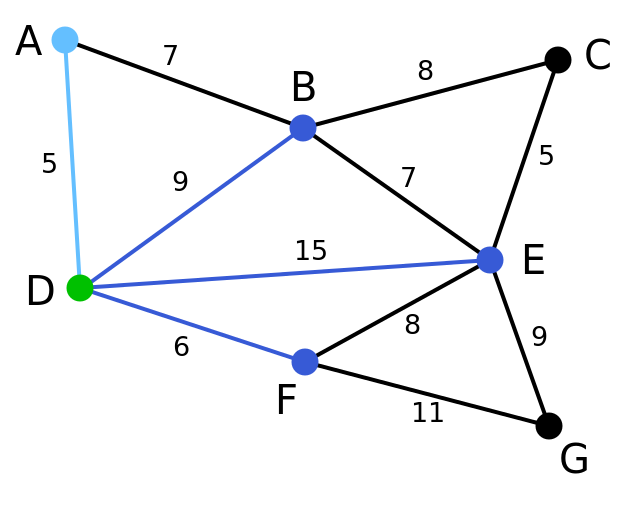
\includegraphics[width=0.24\textwidth]{images/example_prim/prim_1.png}
		\hfill
		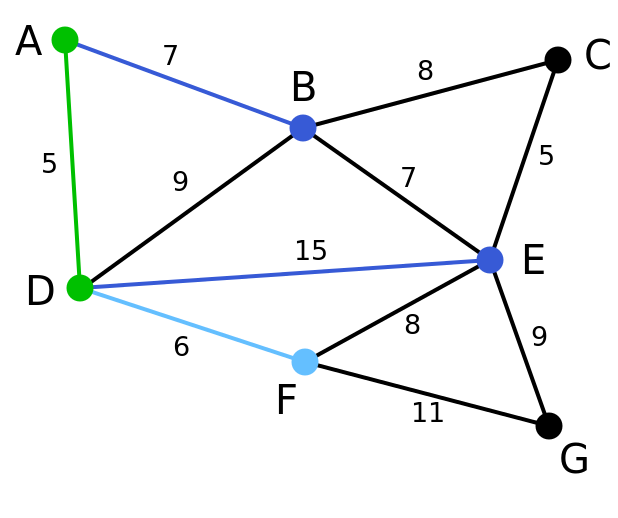
\includegraphics[width=0.24\textwidth]{images/example_prim/prim_2.png}
		\hfill
		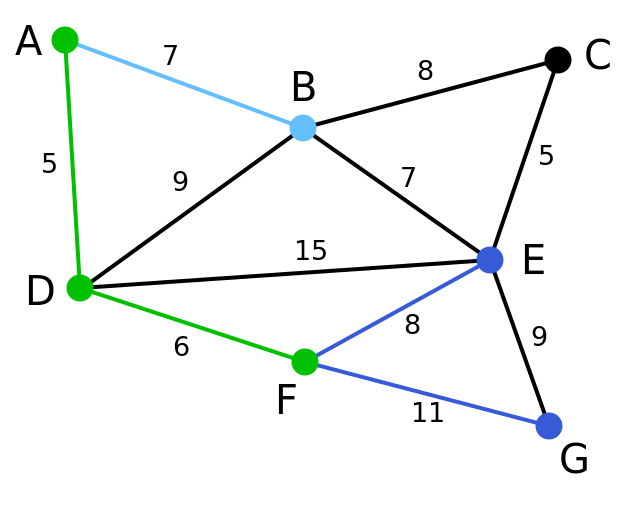
\includegraphics[width=0.24\textwidth]{images/example_prim/prim_3.png}
		\hfill
		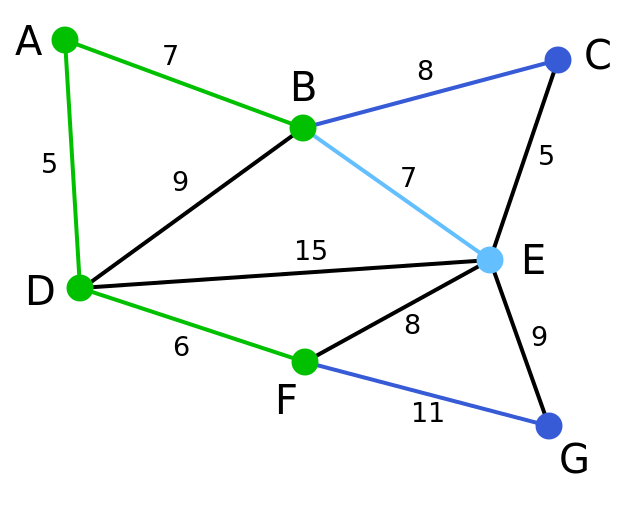
\includegraphics[width=0.24\textwidth]{images/example_prim/prim_4.png}
	\end{figure}
	\begin{figure}[htbp]
		\centering
		\	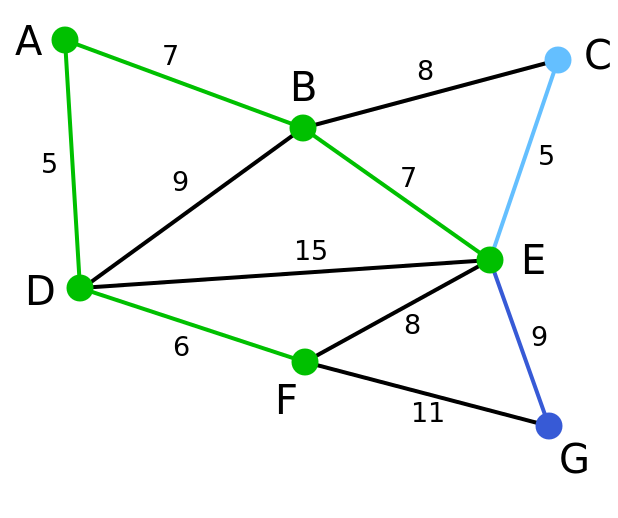
\includegraphics[width=0.24\textwidth]{images/example_prim/prim_5.png}
		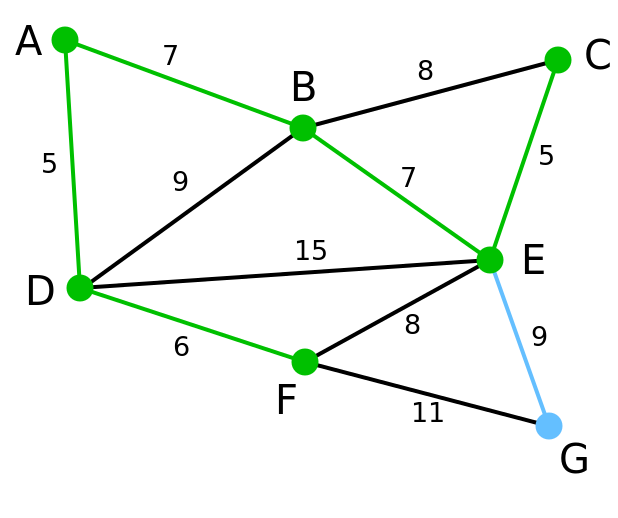
\includegraphics[width=0.24\textwidth]{images/example_prim/prim_6.png}
		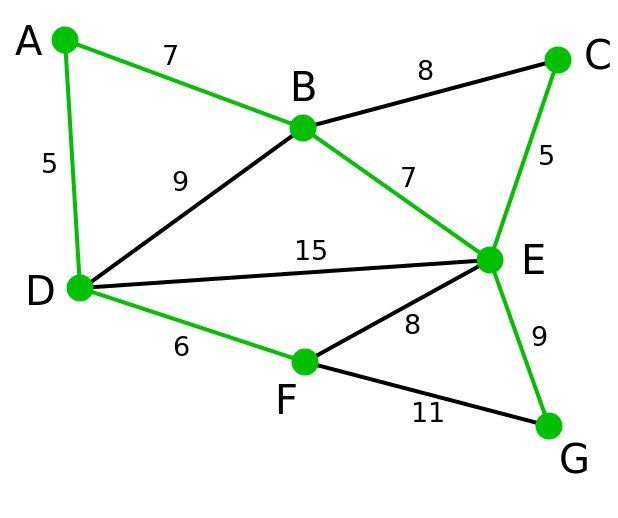
\includegraphics[width=0.24\textwidth]{images/example_prim/prim_7.png}
		\caption{Пример работы алгоритма Прима (7 шагов)}
	\end{figure}
	
	\subsection{Двоичная куча}
	
	В МОЕМ СЛУЧАЕ КУЧА ХРАНИТ ВЕРШИНУ И РАССТОЯНИЕ ДО НЕЁ ТАК ЧТО НАДО ЧУТЬ ПЕРЕДЕЛАТЬ (В ТЕКСТЕ РЕЧЬ О РЕБРАХ)
	
	\hspace{0.5 cm} Для поиска ребра минимального веса требуется структура данных, которая умеет быстро добавлять в себя новые рёбра, удалять использованные рёбра и находить среди рёбер минимальное. 
	
	Для быстрого нахождения минимального элемента существует структура данных, называемая кучей. Кучу можно реализовать несколькими способами, обладающими различным временем работы. В этой главе рассматривается двоичная куча. 
	
	Введём на множестве рёбер отношение порядка так, что ребро с меньшим весом меньше, чем ребро с большим весом. 
	
	Двоичная куча представляет из себя иерархическую структуру, дерево, в котором корнем является самый маленький элемент, а все вершины хранят номер предка. Для каждой вершины дерева выполняется правило: у неё может быть не более 2 вершин, считающих её предком (другими словами, не более 2 детей), кроме того, вершина должна быть меньше, чем её дети. В нашем случае вершинами в куче являются рёбра, и корневой вершиной будет являться ребро с минимальным весом. 
	
	Двоичная куча реализована в алгоритмической части как класс \texttt{BinaryHeap}. Само дерево кучи хранится как вектор \texttt{heap}, хранящий рёбра. В векторе поддерживается следующий инвариант: корень дерева хранится под индексом $0$, а дети вершины под индексом $i$ хранятся под индексами $2i + 1$ и $2i + 2$. Тогда родитель вершины с индексом $i$ будет храниться под индексом $(i - 1) / 2$, деление целочисленное.
	
	Изначально вектор \texttt{heap} пуст, потому что в кучу ещё ничего не добавлено. Добавление в двоичную кучу происходит следующим образом: к уже имеющемуся вектору \texttt{heap} в конце добавляется элемент. Далее, этот элемент по формуле выше находит своего предка и сравнивает себя с ним. Если элемент меньше своего предка, то они меняются местами в векторе \texttt{heap}. Данное действие повторяется для добавленной вершины до тех пор, пока предок не окажется меньше или пока не окажется, что добавленная вершина стала корневой, то есть у неё индекс $0$. Данный алгоритм называется просеиванием вверх и реализуется в методе \texttt{push} класса \texttt{BinaryHeap}. Данная операция имеет сложность $O(\log E)$.
	
	После взятия наименьшего элемента из кучи его следует удалить, потому что он уже использован, и хранить его не имеет смысла. Взятие элемента происходит тривиально, а удаление элемента происходит следующим образом: самый последний элемент кучи встаёт на место самого маленького элемента, то есть занимает индекс $0$. Далее этот элемент меняется местами с наименьшим из своих детей, если ребёнок меньше данной вершины. Это действие повторяется для данной вершины до тех пор, пока у вершины существует ребёнок, меньший её самой. Данный алгоритм называется просеиванием вниз и реализуется в методе \texttt{pop} класса \texttt{BinaryHeap}. Данная операция имеет сложность $O(\log E)$.
	
	Для внедрения данной структуры данных в алгоритм Прима реализована отдельная стратегия в классе \texttt{BinaryHeapStrategy}, которая содержит в себе поля \texttt{dist} и \texttt{used}. Первое является экземпляром класса двоичной кучи, второе является вектором, хранящим $1$ по индексу, соответствующему номеру вершины, если эта вершина уже добавлена в минимальное остовное дерево, и $0$ в противном случае. Добавление в двоичную кучу происходит при помощи метода \texttt{update}. Ключевым является метод \texttt{find\_min}, который берёт минимальный элемент из кучи, и, если он не является использованным, возвращает его. Если его уже использовали, то удаляем этот элемент и берём следующий. 
	
	Теоретическая сложность алгоритма Прима с использованием двоичной кучи составляет $O((E + V) \log V)$, что показывается в [КОРМЕН ВСТАВИТЬ НОМЕР]. 
	
	Пример работы двоичной кучи приведён на рисунке (СДЕЛАТЬ РИСУНОК).
	
	\subsection{Фибоначчиева куча}
	
	\hspace{0.5 cm}
	
	[БОЛЬШЕ ПРО СТРУКТУРУ] Для фибоначчиевой кучи сохраняется инвариант: каждая вершина фибоначчиевой кучи содержит значение, меньшее чем у любого из её детей. Фибоначчиева куча отличается от двоичной тем, что вершина в ней может иметь более двух детей. Кроме того, в фибоначчиевой куче каждая вершина имеет степень. Вершина имеет степень $i$, если она представляет собой вершину степени $i-1$, к которой подвесили вершину степени $i-1$. Вершина степени $0$ --- вершина без детей.
	
	Кроме того, вершине разрешается не иметь одного из детей. Такая вершина называется помеченной. Дети вершин хранятся в циклическом двусвязном списке. Родитель хранит детей как указатель на один из элементов циклического списка. Каждая вершина хранит указатель на родителя. 
	
	Итого, каждая вершина фибоначчиевой кучи хранит в себе следующую информацию:
	\begin{enumerate}
		\item значение;
		\item указатель на родителя;
		\item указатель на одного из детей;
		\item указатель на левого и правого соседа в циклическом списке;
		\item степень вершины;
		\item отметка, является ли вершина помеченной или нет.
	\end{enumerate}
	
	По умолчанию каждая вершина считает левым и правым соседом себя, детей и родителя не имеет, имеет степень $0$ и не является помеченной.
	
	В алгоритмической части вершина фибоначчиевой кучи реализована как подкласс \texttt{Node} класса \texttt{FibonacciHeap}, реализующего логику фибоначчиевой кучи.
	
	\texttt{FibonacciHeap} хранит в себе указатель на минимальный элемент и актуальное число элементов в куче.
	
	Добавление элемента в фибоначчиеву кучу происходит так: создаётся вершина кучи с указанным значением, остальные параметры создаются по умолчанию. Далее эта вершина добавляется как правый сосед минимальной вершины. Указатели на соседей у добавленной вершины, у минимальной и у правого соседа минимальной переставляются с поддержанием структуры. Если добавленная вершина меньше, чем минимальная, или минимальной вершины ещё нет, то добавленная вершина становится минимальной. Добавление элемента реализовано в методе \texttt{push} класса \texttt{FibonacciHeap} и работает за $O(1)$.
	
	Удаление минимального элемента происходит несколько сложнее. Удаляем минимальный элемент, а его детей добавляем в корневой список, то есть в самый верхний циклический список соседей. Если корень остался один, то делаем его минимальным элементом. В противном случае необходимо слить все деревья корневого списка так, чтобы в нём не осталось деревьев с одинаковой степенью. Удаление минимального элемента происходит за $O(\log E)$ и реализовано в методе \texttt{pop} класса \texttt{FibonacciHeap}. 
	
	Слияние деревьев происходит при помощи перебора всех корневых вершин. До перебора создаётся вектор \texttt{degree\_table}, который хранит под индексом $i$ указатель на корневую вершину степени $i$. Перебор происходит так: берём очередную корневую вершину. Если \texttt{degree\_table} хранит в себе указатель на вершину такой же степени, как у очередной вершины, то подвешиваем вершину с меньшим значением к вершине с большим значением, обнуляем значение по этому индексу в \texttt{degree\_table} и увеличиваем степень получившейся вершины, повторяем те же операции с увеличенной степенью. Далее обновляем информацию в \texttt{degree\_table}. Если \texttt{degree\_table} не хранит указатель на вершину такой же степени, то добавляем по этому индексу указатель на текущую вершину. После окончания слияния проходим по всем вершинам корневого списка и ищем минимальный элемент. Слияние деревьев и нахождение нового минимального элемента происходит за $O(\log E)$ и реализовано в приватном методе \texttt{consolidate} класса \texttt{FibonacciHeap}.
	
	В алгоритме Прима часто приходится обновлять веса, с чем фибоначчиева куча справляется за $O(1)$. Обновляем вес у указанной вершины и, если у неё есть родитель с большим значением, вырезаем указанную вершину со всеми её потомками и цепляем её к корневому списку, и обновляем данные у родителя. [ОПИСАТЬ БОЛЕЕ ПОДРОБНО] Обновление веса у вершины реализовано в методе \texttt{decrease\_key} класса \texttt{FibonacciHeap}.
	
	[ОПИСАТЬ КАК ВНЕДРЁНА КУЧА ФИБОНАЧЧИ В АЛГОРИТМ ПРИМА]
	
	[ДОБАВИТЬ ПРИМЕР РАБОТЫ ФИБОНАЧЧИЕВОЙ КУЧИ С РИСУНКАМИ]
	
	\newpage
	
	\section{Вычислительный эксперимент}
	
	\subsection{Генерация данных}
	
	\hspace{0.5 cm} 
	
	Сравнительный анализ алгоритмов Прима и Краскала требует измерения времени их работы на графах с различным количеством вершин и рёбер, причём необходимо исследовать различные соотношения количества вершин и рёбер, так как алгоритмы и их различные оптимизации могут показывать различные результаты на плотных и разреженных графах.
	
	Поставленная задача сводится к генерации графа случайной структуры и со случайными весами рёбер по заданному количеству вершин и рёбер. При этом подразумевается, что можно построить граф с заданными параметрами, то есть что количество вершин и рёбер задано корректно. Логику генерации графа реализует метод fill класса Edges. В программе использование этого метода происходит следующим образом: у экземпляра класса Edges после его создания с заданными параметрами вызывается метод fill, который заполняет данный граф рёбрами описанным ниже образом. 
	
	Во-первых, так как граф обязан быть связным, все вершины последовательно соединяются рёбрами, образуется цикл. Во-вторых, происходит случайный выбор двух различных вершин. В случае, если между вершинами нет ребра, генерируется ребро случайного веса между этими вершинами, и если текущее количество рёбер не превысило указанное при создании экземпляра класса количество рёбер, происходит повторение той же операции, начиная с выбора двух различных вершин. Если ребро между двумя выбранными вершинами существует, то две вершины выбираются заново. 
	
	В алгоритме, описанном выше, все вершины выбираются равновероятно, и вес генерируемого ребра выбирается случайным образом из равномерного распределения от 0 до 1. 
	
	Важно отметить, что проверка того, сгенерировано ли ребро или нет, происходит при помощи хэш-таблицы, реализованной в стандартной библиотеке языка программирования C++, которая при помощи вычисления хэшей добавляет, удаляет и проверяет, лежит ли в ней указанный элемент, амортизированно за O(1).
	
	\subsection{Измерение времени работы алгоритмов}
	
	\hspace{0.5 cm}
	
	Измерение времени работы реализовано внутри алгоритмов. То есть функции, реализующие алгоритмы Прима и Краскала, в том числе засекают время собственной работы и возвращают его вместе с получившимся графом. Такая реализация выбрана из-за того, что помимо работы непосредственно алгоритмов происходят мелкие операции, такие как передача в функцию параметров, инициализация классов, которые к алгоритмам не относятся, но при небольшом количестве рёбер и вершин могут существенно влиять на показатели скорости работы. 
	
	Функции run\_kruskal\_test, run\_prim\_binary\_test, run\_prim\_fibonacci\_test, \\run\_prim\_vector\_test реализуют внутри себя генерацию данных для сравнительного анализа: перебирается количество вершин с указанными границами, для фиксированного количества вершин по заданной формуле подсчитывается количество рёбер и генерируется граф указанного размера. Для него запускается соответствующий алгоритм, после чего в указанный файл записывается время работы алгоритма и соответствующие параметры. Формулы подсчёта количества рёбер в зависимости от количества вершин выбраны следующие:
	
	1) E = \(2V\)
	
	2) E = \( V\sqrt{V}\)
	
	3) E = \(V^2~/~4\) \\
	где E — количество рёбер в графе, а V — количество вершин в графе.
	
	Количество вершин перебирается от 300 до 4000 с шагом в 50 вершин.
	
	\subsection{Сравнительный анализ}
	
	\hspace{0.5 cm}
	
	Напомним, что сравнительный анализ производится для 4 алгоритмов:
	
	- алгоритм Краскала с системой непересекающихся множеств со сложностью работы $O(E \log E)$;
	
	- алгоритм Прима с вектором со скоростью работы $O(V^2 + E)$;
	
	- алгоритм Прима с двоичной приоритетной очередью со скоростью работы $O((V + E) \log V)$;
	
	- алгоритм Прима с фибоначчиевой приоритетной очередью со скоростью работы $O(E + V \log V)$,
	
	где V — количество вершин, E — количество рёбер.
	
	Сравнительный анализ указанных выше алгоритмов производится при помощи языка программирования Python и библиотеки matplotlib, позволяющей строить графики. Всего написано 2 программы на Python.
	
	Первая программа сравнивает абсолютную скорость работы алгоритмов при различном соотношении количества вершин и количества рёбер. Она считывает данные из файлов, содержащих информацию из прошлого пункта, после чего строит графики зависимости времени работы алгоритма от количества вершин для различных соотношений. Результат работы программы представлен на рисунке [ДОБАВИТЬ РИСУНОК]
	
	%\begin{figure}[htbp]
	%	\centering
	%	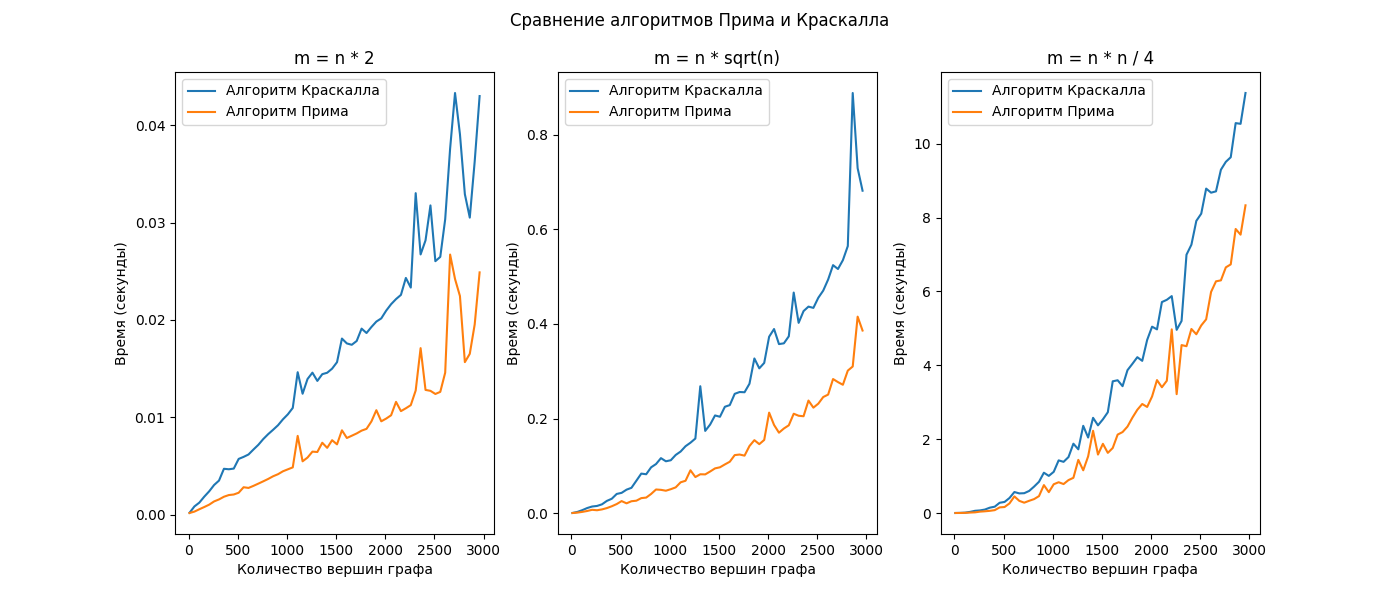
\includegraphics[width=1.0\textwidth]{images/algorithm_comparasion.png}
	%	\caption{Сравнение алгоритмов}
	%\end{figure}
	
	[ДОБАВИТЬ АНАЛИЗ РИСУНКА]
	
	Вторая программа проверяет соответствие асимптотической сложности алгоритмов реальному времени работы алгоритмов. Программа считывает данные из файлов, содержащих информацию из прошлого пункта, после чего строит графики зависимости отношения реального времени работы алгоритмов к оценке сложности от количества вершин графа для каждого из алгоритмов. Результат работы программы представлен на рисунке [ДОБАВИТЬ РИСУНОК]
	
	%\begin{figure}[htbp]
	%	\centering
	%	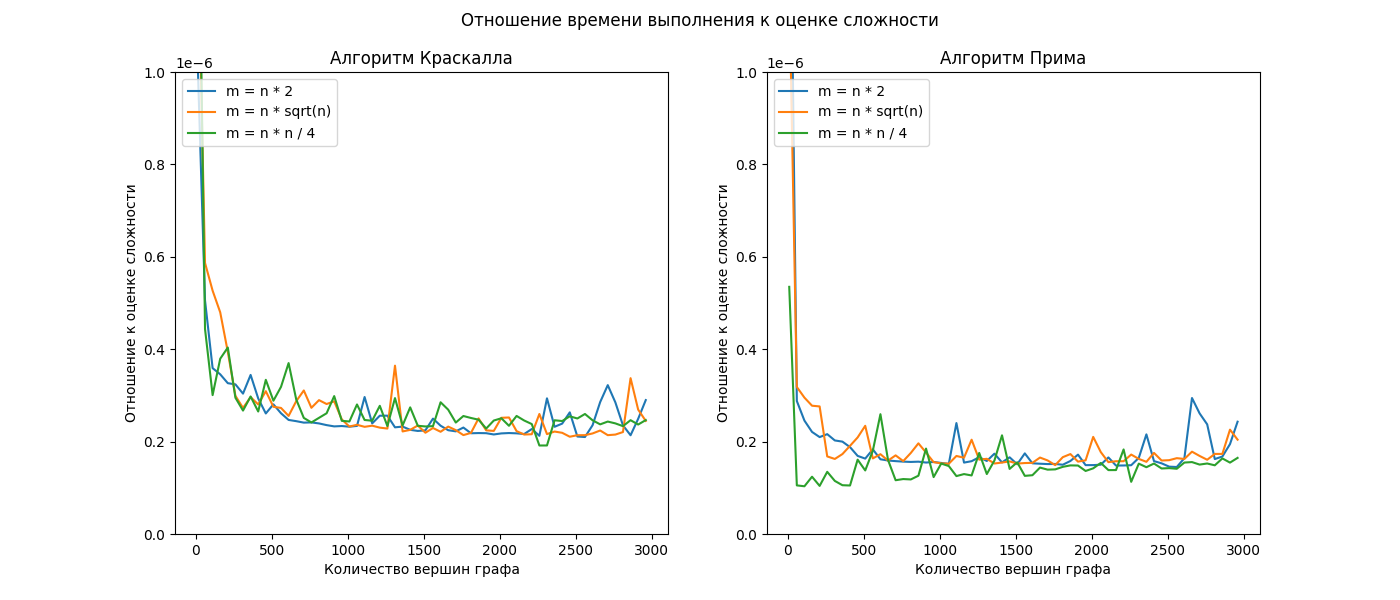
\includegraphics[width=1.0\textwidth]{images/big_o_analysis.png}
	%	\caption{Отношение времени выполнения к оценке сложности}
	%\end{figure}
	
	[ДОБАВИТЬ АНАЛИЗ РИСУНКА]
	
	\newpage
	
	\section{Заключение}
	
	\subsection{Рассмотренные задачи}
	
	\hspace{0.5 cm}
	
	В выпускной квалификационной работе рассмотрены следующие задачи:
	
	- изучить алгоритмы Краскала и Прима;
	
	- изучить двоичную приоритетную очередь;
	
	- изучить фибоначчиеву приоритетную очередь;
	
	- изучить систему непересекающихся множеств;
	
	- реализовать алгоритмы Краскала и Прима;
	
	- реализовать оптимизации алгоритмов Прима и Краскала;
	
	- провести сравнительный анализ алгоритмов Краскала и Прима.
	
	\subsection{Основные результаты работы}
	
	\hspace{0.5 cm}
	
	В выпускной квалификационной работе были достигнуты следующие результаты:
	
	- реализованы алгоритмы Краскала и Прима на языке программирования C++;
	
	- независимо с использованием шаблонов реализована двоичная приоритетная очередь, вследствие чего её реализацию можно использовать в других работах;
	
	- независимо с использованием шаблонов реализована фибоначчиева приоритетная очередь, реализация которой может быть использована в других работах;
	
	- независимо реализована система непересекающихся множеств, реализация которой может быть использована в других работах;
	
	- код реализации алгоритмов является расширяемым, что позволяет в будущем рассмотреть дополнительные оптимизации алгоритмов, в том числе добавление других алгоритмов;
	
	- была написана программа на языке программирования Python, строящая графики скорости выполнения алгоритмов Краскала и Прима и их различных оптимизаций;
	
	- был проведён сравнительный анализ алгоритмов Краскала и Прима и их оптимизаций, в том числе сравнительный анализ скорости их работы.
	
	\subsection{Репозиторий с реализацией}
	
	\hspace{0.5 cm}
	
	Процесс разработки алгоритмов Прима, Краскала, их оптимизаций, а также кода, необходимого для их сравнительного анализа, фиксировался в открытом репозитории GitHub по следующей ссылке: \href{https://github.com/dan1lka257/graduate_work}{\textcolor{blue}{\underline{GitHub}}}.
	
	Важно отметить, что стабильные версии добавлены в ветку main, в то время как промежуточные версии добавлены в ветку develop. Стабильные и промежуточные версии помечены тегами версий, что позволяет более удобно прослеживать процесс разработки.
	
	\newpage
	
	\section{Список литературы}
	
	[НЕАКТУАЛЬНЫЙ СПИСОК ЛИТЕРАТУРЫ]
	\begingroup
	\renewcommand{\section}[2]{}
	\begin{thebibliography}{10}
		
		\bibitem{boruvka1926}
		Borůvka O.
		\textit{O jistém problému minimálním}.
		Práce Moravské Přírodovědecké Společnosti, 1926.
		Vol. 3, No. 3, pp. 37--58.
		
		\bibitem{cormen2009}
		Cormen T. H., Leiserson C. E., Rivest R. L., Stein C.
		\textit{Introduction to Algorithms}.
		3rd ed. MIT Press, 2009.
		
		\bibitem{cormen2022}
		Cormen T. H., Leiserson C. E., Rivest R. L., Stein C.
		\textit{Introduction to Algorithms}.
		4th ed. MIT Press, 2022.
		
		\bibitem{harrington2002}
		Harrington J. L.
		\textit{Object-oriented C++ Data Structures for Real Programmers}.
		Morgan Kaufmann, 2002.
		
	\end{thebibliography}
	\endgroup
\end{document}